\section{Problem Statement and System Overview}
\label{sec:overview}

This section briefly describes KDEEB algorithm, followed by a discussion of inconsiderate settings when applied to OD trails in urban traffic.
An overview of RAEB is presented at the end.

\begin{figure}[t] 
	\centering
	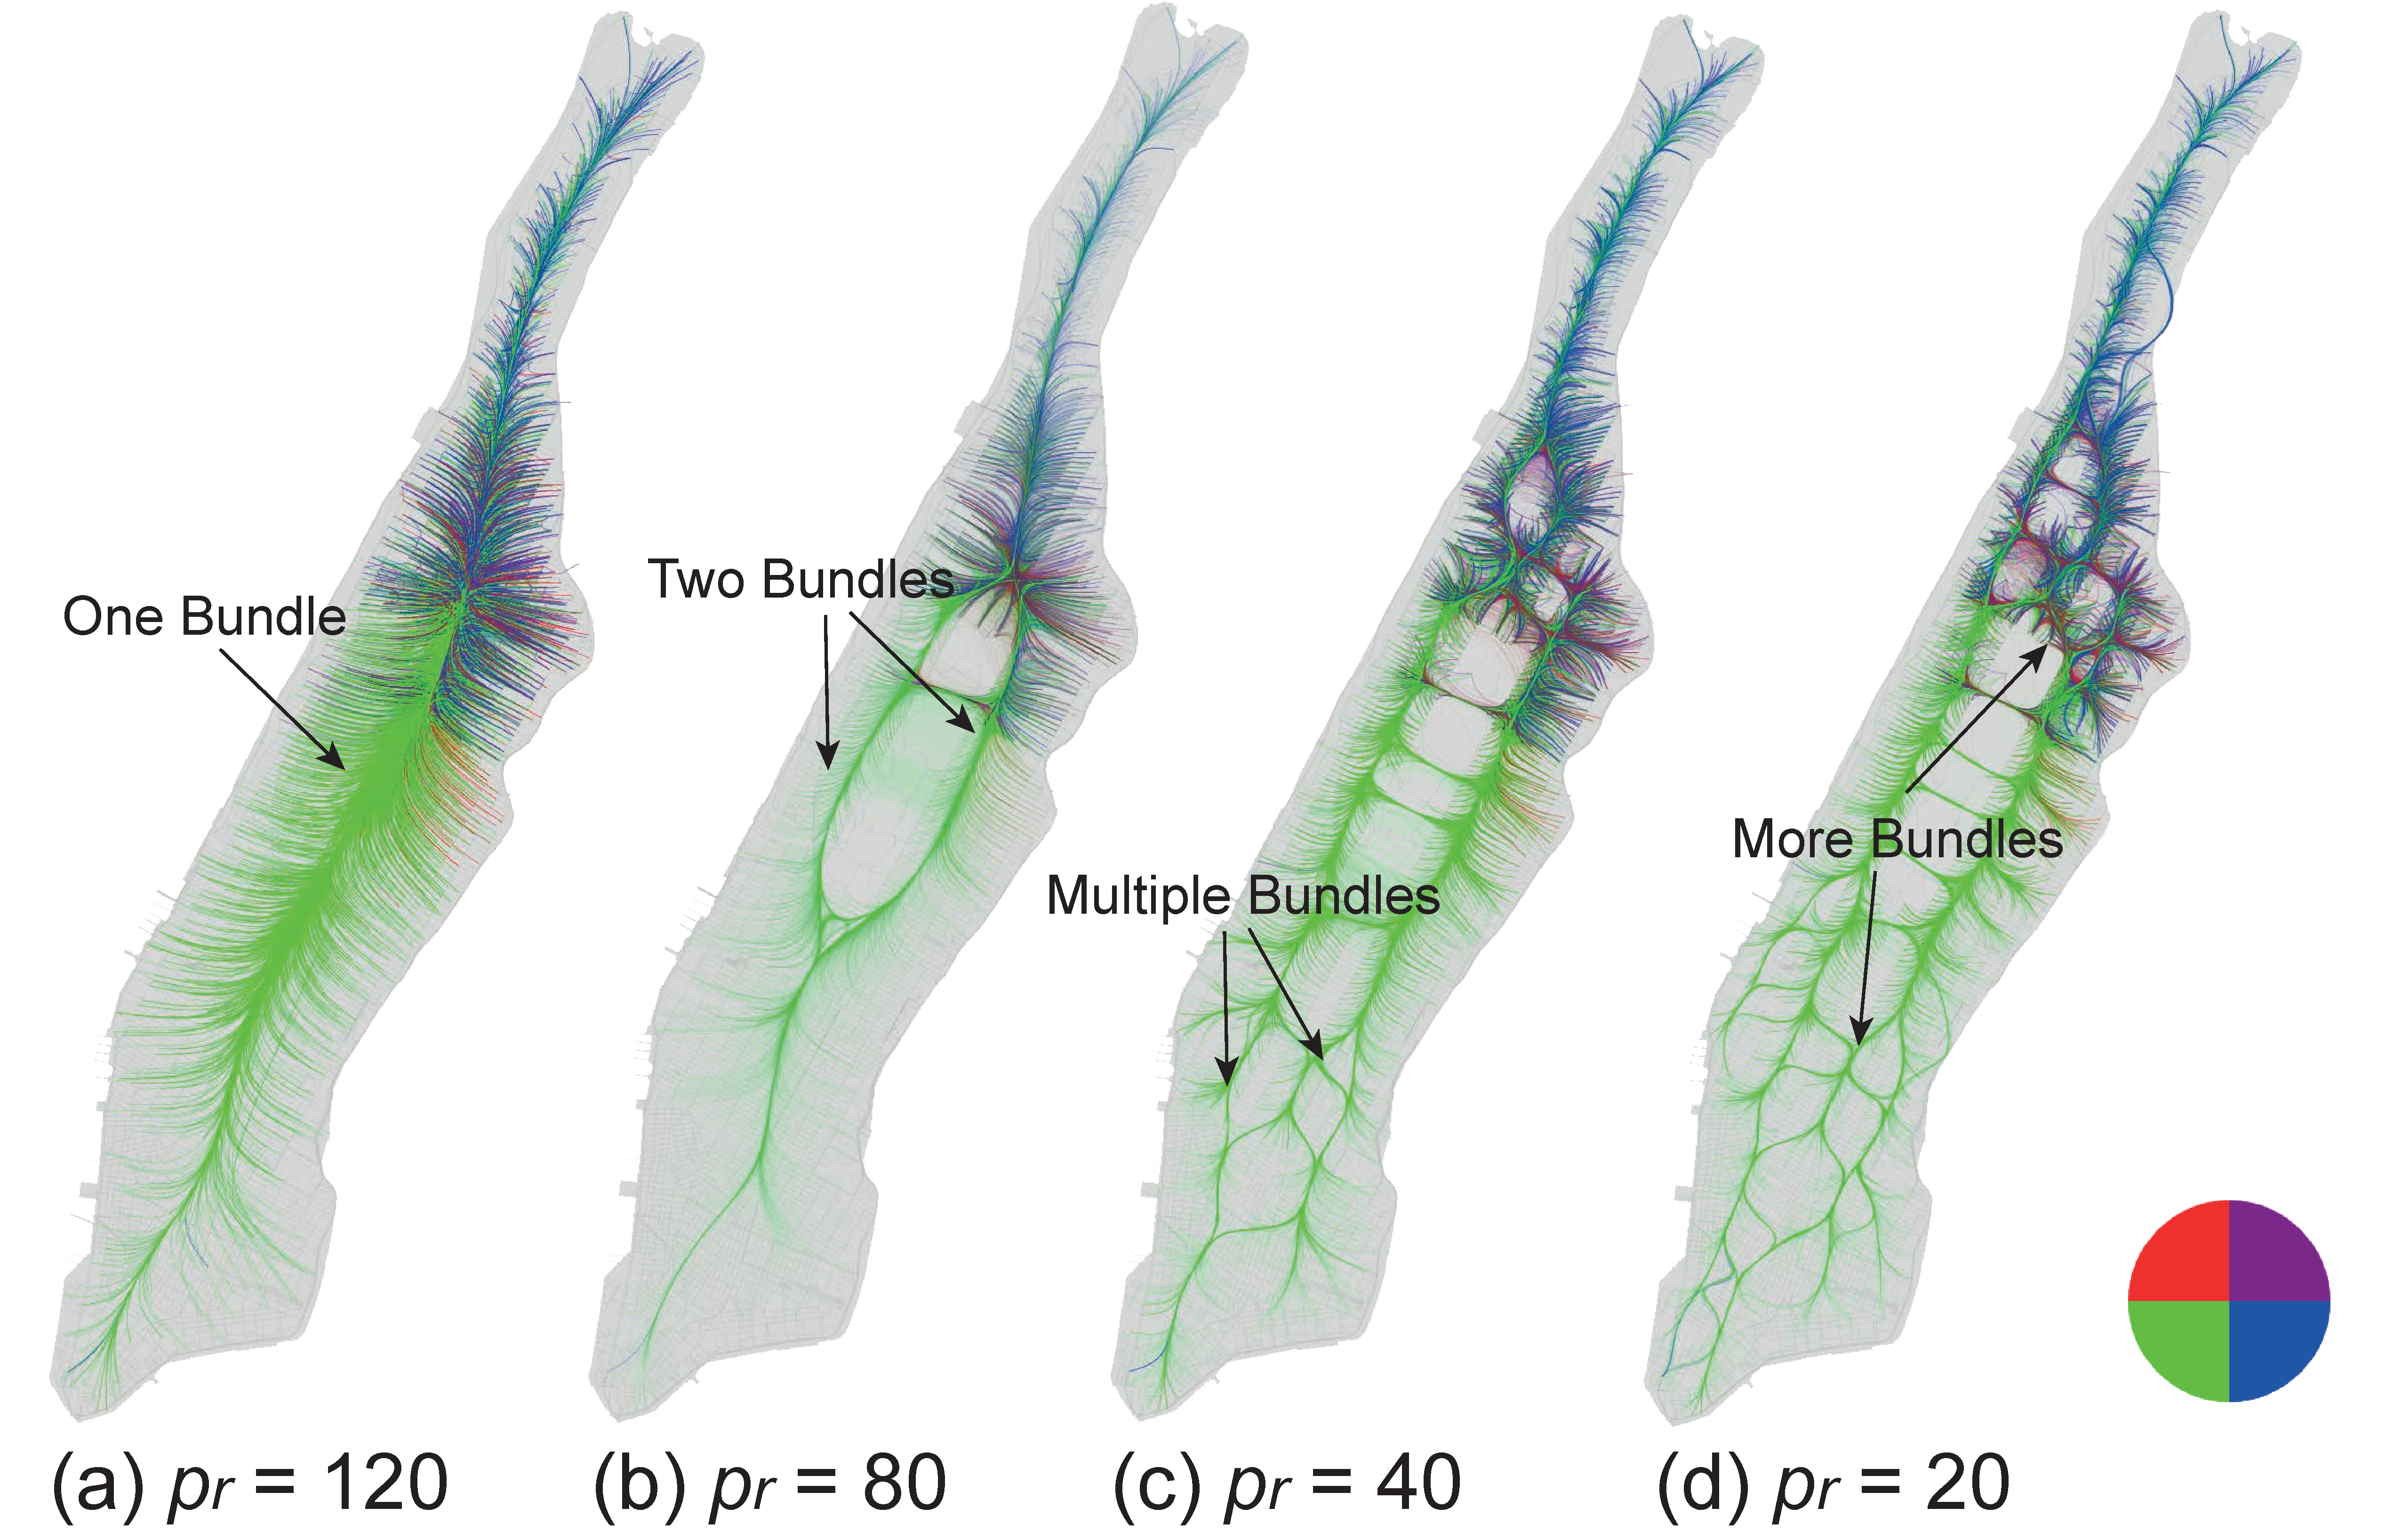
\includegraphics[width=0.495\textwidth]{figure/edgebundling/fig2_kernel_size/kernel_size}
	\vspace{-5mm}
	\caption{KDEEB applied to taxi trips in Manhattan with different kernel sizes $p_r$: (a) 120, (b) 80, (c) 40, and (d) 20.
	More detailed bundles are generated with smaller $p_r$.}
	\label{fig:kernel_size}
	\vspace{-5mm}
\end{figure}

%%%%%%%%%%%%%%%%%%%%%%%%%%%%%%%%%%%%%%%%%%%%%%%%%%%%%%%%%%%%%%%%%%%%
%%%%%%%%%%%%%%%%%%%%%%%%%%%%%%%%%%%%%%%%%%%%%%%%%%%%%%%%%%%%%%%%%%%%

\subsection{KDEEB Algorithm}
\label{ssec:kdeeb}
KDEEB is a fast edge bundling method for visualizing dense graphs.
It employs a general pipeline with edge sampling, splatting, gradient estimation, edge advection, and bundle smoothing.
In edge sampling step, an edge $\textbf{e}_i$ is divided into uniformly-sampled polylines, i.e., $\textbf{e}_i = \{\textbf{x}_j\}$, with user-given sampling step $\sigma$.
After that, KDEEB computes a density map $\rho : \mathbb{R}^2 \rightarrow \mathbb{R}^+ $as

\vspace{-4mm}
\begin{equation}\label{eq:kernel_density_estimation}
\rho(\textbf{x} \in \mathbb{R}^2) = \sum_{\textbf{y} \in D} K (\frac{\|\textbf{x}-\textbf{y}\|}{p_r})
\end{equation}

where $K$ is a parabolic radial kernel and $p_r$ is kernel radius.
Next, each edge sampling site $\textbf{x}_j$ is advected to a new position $\textbf{x}'_j$ as:

\vspace{-5mm}
\begin{equation}\label{eq:advecting_points}
\textbf{x}'_j = \textbf{x}_j + p_r \frac{\nabla \rho}{||\nabla \rho||}
\end{equation}

Finally, a smoothing function is applied on $\textbf{x}_j$ to remove jitters created by the advection step.
These steps are repeated $p_n$ times until stable bundles are generated.

\vspace{2mm}
\noindent
\textit{Parameter Setting}.
KDEEB requires several parameters to be preset by users.
Following settings are recommended~\cite{van2016cubu}:
\begin{itemize}

\item 
Kernel radius $p_r$: Initial value set to 5\% of graph drawing size.
A constant decay ratio $\lambda$ in [0.5, 0.9] is applied to $p_r$ at each bundling iteration $n$.

\item
Bundling iteration $p_n$: An integer in between 10 to 15.

\end{itemize}

\begin{figure*}[t]
	\centering
	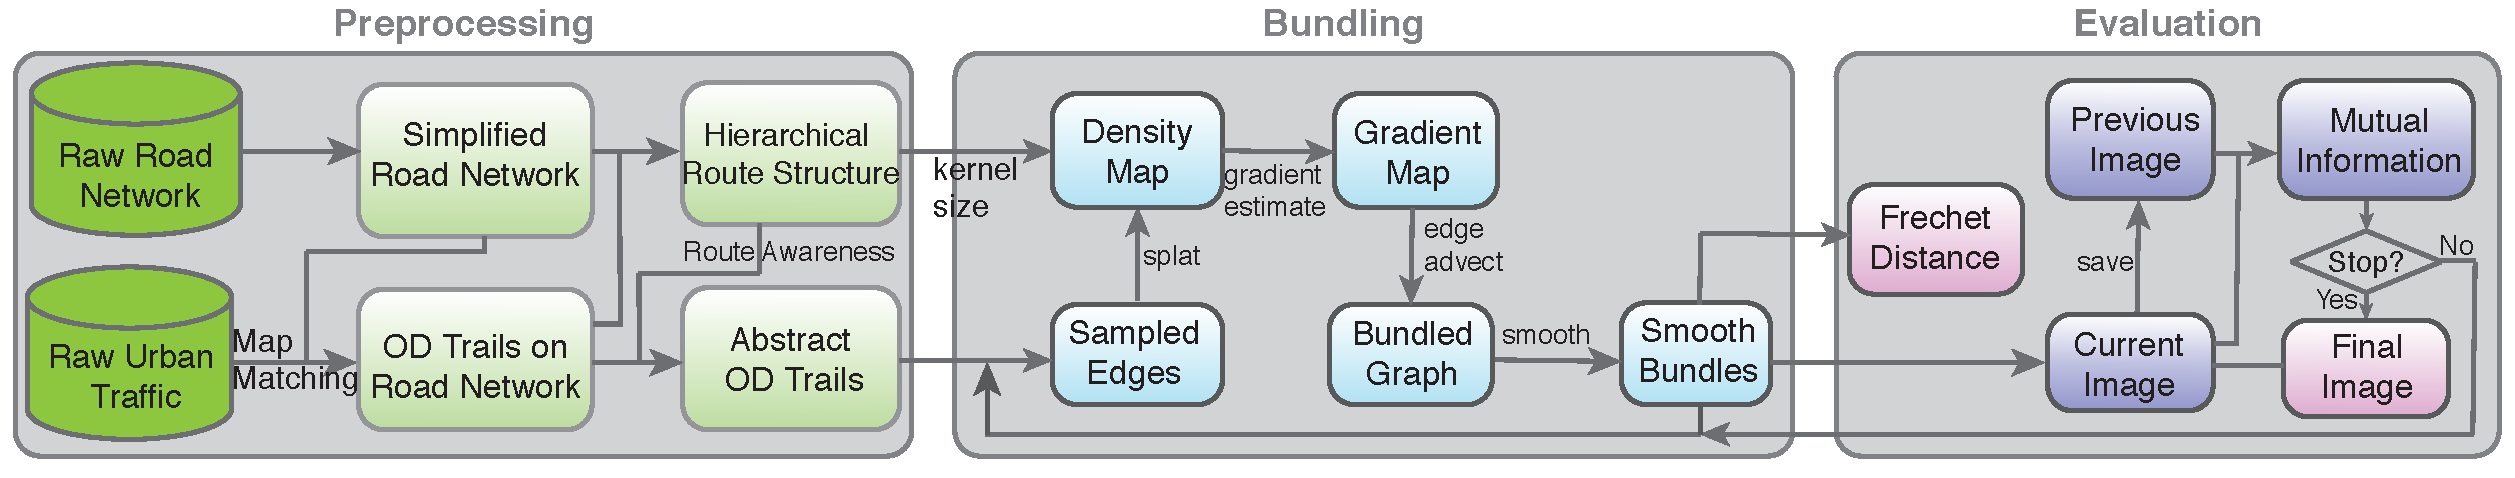
\includegraphics[width=0.995\textwidth]{figure/edgebundling/fig3_framework/framework2.pdf}
	\vspace{-3mm}
	\caption{Overview of RAEB pipeline.
	Our method mainly consists of three phases: \textit{Preprocessing} for creating a proper initial layout, \textit{Bundling} for bundling input OD trails, and \textit{Evaluation} for generating a stable bundle structure.}
	\label{fig:framework}
	\vspace{-4mm}
\end{figure*}

%%%%%%%%%%%%%%%%%%%%%%%%%%%%%%%%%%%%%%%%%%%%%%%%%%%%%%%%%%%%%%%%%%%%
\subsection{Problem Identification}
The parameter settings are recommended for general graphs that consist of fixed nodes and connections between them.
For such a graph, it is free to manipulate node connections into smooth polylines.
However, when applied to OD trails in urban traffic data, KDEEB encounters the following issues.

\begin{itemize}
\item
\textit{P1: Non-optimal Kernel Radius}.
Kernel radius $p_r$ in KDEEB is solely based on graph drawing size, while ignores geometric properties of road network.
Figure~\ref{fig:kernel_size} presents KDEEB results generated with different kernel sizes for taxi trips in Manhattan: 120, 80, 40, and 20 in (a) - (d), respectively.
Sizes for graph drawing are all 720$\times$1440, thus KDEEB would recommend $p_r$ = 80 as 5\% of graph graphing size.
However, smaller $p_r$ generate more detailed and visual appealing bundles, comparing Figure~\ref{fig:kernel_size}(b) to (c) \& (d).
This happens because most space in graph drawing are not utilized, due to the long and thin shape of Manhattan island.
In addition, urban traffic can unevenly spread in a city, such as Shenzhen taxi data (Section~\ref{ssec:study3}), making small $p_r$ preferable.

\vspace{1mm}
\item
\textit{P2: Road Neglect}.
Urban traffic are moving along roads in a city, thus OD trails should be constrained to roads in a city.
However, KDEEB represents each OD connection with a direct line, while ignores information about the road network.
Thus, resulting bundles can be displaced far away from the roads.
This can cause impression of traffic moving in wrong positions, such as those bundles in between Manhattan and Brooklyn (Section~\ref{ssec:study1}).
The displacements can also add difficulty to mentally map original OD trails with resulting bundle lines.
\end{itemize}

\vspace{2mm}
\noindent
Besides, KDEEB lacks a quantitative method to automatically terminate bundling iterations.

\begin{itemize}
\item
\textit{P3: Preset Bundling Iterations}.
KDEEB is an image-based edge bundling method. 
Most of these bundling methods generate bundling results in an iterative way. 
The number of bundling iterations $p_n$ is preset based on practical experience: 10 in KDEEB~\cite{hurter2012graph}, while 15 in CUBu~\cite{van2016cubu}.
The numbers are chosen because tight and stable bundles are generated.
However, these conditions are rather subjective, which can vary among individuals and may be affected by other parameters like image size and sampling step.
\end{itemize}

%%%%%%%%%%%%%%%%%%%%%%%%%%%%%%%%%%%%%%%%%%%%%%%%%%%%%%%%%%%%%%%%%%%%
\subsection{RAEB Overview}
We develop route-aware edge bundling (RAEB), a comprehensive edge bundling method specifically designed for visualizing OD trails in urban traffic.
As illustrated in Figure~\ref{fig:framework}, RAEB pipeline mainly consists of three parts: \textit{Preprocessing}, \textit{Bundling}, and \textit{Evaluation}.

In \textit{Preprocessing}, RAEB first generates a simplified road network from the input one such as open street map (OSM).
Raw OD trails are mapped onto simplified road network using map matching algorithms.
Together with urban traffic information, simplified road network can be organized in a hierarchical route structure.
OD trails can be abstracted accordingly depending on a new parameter of route awareness defined by users.
A value for kernel size is also measured based on geometric property of the route structure.

The abstract OD trails are passed into \textit{Bundling} stage as input graph.
Bundling process is an image-based approach similar to KDEEB workflow.
Specifically, we discard the preset parameter of bundling iteration $p_n$ in KDEEB.
Instead, we introduce a new parameter of bundling stability, which is measured as normalized mutual information between images generated by two consecutive iterations.
The measurement is done in the \textit{Evaluation} stage.
If bundling stability reaches a threshold, we terminate the bundling iteration and export a final image.
Besides, we measure Fréchet distance between generated bundles to OD trails mapped on the road network.
The measurement complements final image with a quantitative metric that reveals quality of a bundling method.